\documentclass{article}
% Minimal CJK support: the reproduction command in \S\ref{sec:verify} cites a
% directory whose name is in Chinese; scheme=plain keeps the document a plain
% English article while the Fandol fonts render those directory-name glyphs.
\usepackage[UTF8, scheme=plain, fontset=fandol]{ctex}
% Draft (2026-10-10); English version of the Chinese draft (same day).
% Structure: each section presents Phenomenon -> Theorem/lemma -> Hypotheses ->
% Lean formalization -> Conclusion.
% Figures carried over from the working corpus (base-point circles / four
% readings / argument rectangle / fourteen-layer overview).
\usepackage[margin=1in]{geometry}
\usepackage{amsmath,amssymb,amsthm}
\usepackage[singlelinecheck=false]{caption}
\usepackage{array}
\usepackage[hidelinks]{hyperref}
\usepackage{tikz}
\usetikzlibrary{arrows.meta,positioning}
\usepackage[numbers,sort&compress]{natbib}
\emergencystretch=3em
% Typesetting of machine-checked names: disable hyphenation inside \texttt
% (so that no hyphen is inserted into machine-checked names or file names at
% line breaks), and allow breaks at \_ (long machine-checked names cannot be
% broken otherwise, which causes overfull or stretched lines)
\let\ttfamilyOrig\ttfamily
\renewcommand{\ttfamily}{\ttfamilyOrig\hyphenchar\font=-1 }
\let\underscoreOrig\_
\renewcommand{\_}{\underscoreOrig\allowbreak}

\newtheorem{theorem}{Theorem}[section]
\newtheorem{lemma}[theorem]{Lemma}
\newtheorem{corollary}[theorem]{Corollary}
\newtheorem{proposition}[theorem]{Proposition}
\newtheorem{definition}[theorem]{Definition}
\newtheorem{remark}[theorem]{Remark}

\newcommand{\C}{\mathbb{C}}
\newcommand{\R}{\mathbb{R}}
\newcommand{\Z}{\mathbb{Z}}
\newcommand{\N}{\mathbb{N}}
\newcommand{\GG}{\Gamma}
\newcommand{\zt}{\zeta}
\newcommand{\Lam}{\Lambda}
\newcommand{\Xchi}{\chi}

\title{An Observation Plane for the Riemann Hypothesis:\\
Judgement Completeness and the Open Reading Constraint}
\author{Anonymous}
\date{\today}

\begin{document}
\maketitle

\begin{abstract}
The Riemann hypothesis asserts that all non-trivial zeros of $\zt$ lie on
the critical line $\Re s=1/2$. This paper proves nothing; it does two
things: it restates this assertion on a newly constructed observation
plane, and it states, item by item, which parts of the restatement are
machine-verified and which remain open. The construction has two steps.
The first is a base-point migration: the operator $T(z)=1/(z-i)-1$ turns
the critical line into the unit circle $|T|=1$, and gives the exact mark
$i^{1/(2i)}=e^{\pi/4}$ of this line in the new coordinates. The second
step rotates the coordinate axes by $45^\circ$, producing fold
coordinates $(u,v)$ equivalent to the standard complex coordinates. On
this observation plane, three coordinate properties of the projection
$d=\sqrt2(\Re s-\frac12)$ are verified: the critical line is mapped to a
single point; no point off the critical line is mapped to that point; and
the definition of the projection does not involve $\zt$. On top of this,
judgement completeness is verified: for every zero in the strip, ``on the
critical line'' and ``projection reading zero'' are equivalent,
zero-ness itself is characterized by the two projection components of
the value, and the position along the line is never used. From these
equivalences, the Riemann hypothesis is equivalent to a universal
statement: the projection reading of every zero in the strip is zero.
The equivalences are verified in Lean~4; the universal statement remains
open. Every claim in the paper compiles under Lean~4 and mathlib
(0 error, 0 \texttt{sorry}), and no axioms beyond those of mathlib are
introduced; classical results that are not machine-verified are marked
KNOWN and given references. The paper contains four figures.
\end{abstract}

\section{Introduction: the reduction chain and its boundary}
\label{sec:intro}

\paragraph{Phenomenon.} The usual form of the Riemann hypothesis is: all
non-trivial zeros of $\zt$ lie on the critical line $\Re s=1/2$
\cite{riemann1859, edwards1974, ivic1985}. Around this statement, the
classical theory has already produced several families of mutually
equivalent restatements, for example the reflection pairing of zeros
about the critical line, the absence of zeros outside the critical strip,
and the contrapositive form ``the hypothesis fails if and only if an
off-line zero exists'' \cite{titchmarsh}. The companion assembly work has
written this reduction chain step by step as Lean~4 declarations. The
last step of the chain is ``an off-line zero yields a contradiction'';
for the known families of bridges (Euler product, functional equation,
phase, growth), this step does not go through: an off-line zero drags
along the four zeros of its reflection orbit, and bridges whose input
condition is $\zt\ne0$ cannot be used anywhere on that orbit (the
verification is given in \S\ref{sec:diag}).

\paragraph{Theorem/lemma (cited).} Two verified equivalence items (both
machine-checked versions of standard facts) reduce the scope of the
problem to ``whether an off-line zero exists inside the critical strip'':
\begin{itemize}
\item \texttt{rh\_iff\_all\_zeros\_on\_line\_in\_strips} (proof.lean):
the Riemann hypothesis holds if and only if for every $T\ge0$, every zero
in the strip ($0\le\Re\le1$, $|\Im|\le T$) satisfies $\Re=1/2$;
\item \texttt{rh\_failure\_iff\_offline\_common\_zero}
(zeta\_rh\_oddeven\_iso.lean): the hypothesis fails if and only if there
exists an off-line zero in the strip ($0<\Re<1$, $\Re\ne1/2$,
$\Im\ne0$).
\end{itemize}

\paragraph{Hypotheses.} Absence of zeros outside the strip and the
symmetry of the functional equation are classical; we cite verified
versions. Every classical result that is not machine-verified is marked
KNOWN at its point of use and given a reference.

\paragraph{Lean formalization.} The reduction items cited in this section
are distributed over \texttt{proof.lean}, \texttt{ValueBridge.lean} and
\texttt{zeta\_rh\_oddeven\_iso.lean}, all with 0 \texttt{sorry}. The
counting equivalence (the Riemann hypothesis holds if and only if the
number of zeros on the line equals the number of zeros in the strip,
\texttt{rh\_iff\_N0\_eq\_N}, ValueBridge.lean) reappears in
\S\ref{sec:equivalence}.

\paragraph{Conclusion.} The task can thus be stated in one concrete
sentence: build an observation surface on which ``whether a zero lies on
the critical line'' is fully decided, and on which ``all zeros lie on the
line'' becomes a universal statement about this surface. This paper does
this, and writes down the boundary as well. Each section of the paper
gives five parts in order: phenomenon, theorem/lemma, hypotheses, Lean
formalization, conclusion.

The contributions of this paper are listed in three layers.
\begin{itemize}
\item Mathematical layer (organization of known material): the
observation plane and the fold coordinates (a linear change of basis of
the standard coordinates, \S\ref{sec:migration} to \S\ref{sec:plane});
the reading-form equivalence of the Riemann hypothesis, together with
the counting and common-vertical-line equivalences
(\S\ref{sec:equivalence}).
\item Formalization layer (the machine-verified results of this draft):
the Lean~4 verification of the constructions and of the equivalence chain
above (\S\ref{sec:verify}); the precise form of judgement completeness:
for every zero in the strip, being on the line and the reading vanishing
are true together and false together (\S\ref{sec:anchors} and
\S\ref{sec:complete}).
\item Methodological layer (diagnosis and calibration of this draft): the
two-level calibration of judgement (the individual judgement is complete,
the universal judgement is open, and there is no independent intermediate
level; remark at the end of \S\ref{sec:equivalence}); the structural
diagnosis and the boundary of the remaining step (\S\ref{sec:diag}).
\end{itemize}

\section{Base-point migration: the critical line is the unit circle}
\label{sec:migration}

\paragraph{Phenomenon.} In standard coordinates the critical line is the
straight line $\Re s=1/2$, unrelated to the origin of the reals; the
functional-equation reflection $s\mapsto1-\bar s$ has its fixed points on
this line. The construction takes its base points from the equidistance
structure of this line: the critical line is the perpendicular bisector
of the base points $i$ and $1+i$
(\texttt{critical\_line\_equidistant\_basepoint\_i}), and also the
perpendicular bisector of the origin $0$ and the unit point $1$
(\texttt{on\_line\_iff\_equidistant\_base\_one}). To move the observation
position onto this line, take the operator
\[
  T(z)=\frac{1}{z-i}-1
\]
(this is a M\"obius transformation: a reciprocal and a translation
composed; first reciprocal about the centre $i$, then translate by $-1$).
The modulus of $T$ is the ratio of the distances to the two base points
$|T(z)|^2=|z-1-i|^2/|z-i|^2$ (\texttt{T\_normSq\_ratio}), and equals $1$
on the equidistance line: the critical line becomes the unit circle
$|T|=1$ in the new coordinates; reflection corresponds to inversion in
the unit circle; the real number $0$ is no longer a special point
($T(0)=-1+i$, outside the circle). The exact position of this line in the
new coordinates is the mark $i^{1/(2i)}=e^{\pi/4}$.

\paragraph{Theorem/lemma.} Three verified results:
\begin{theorem}[Base-point migration]
\label{thm:migration}
For $z\ne i$: $|T(z)|^2=1$ if and only if $\Re z=1/2$
(\texttt{T\_normSq\_eq\_one\_iff}); for $z\ne i,\,1+i$:
$T(1-\bar z)=1/\overline{T(z)}$, i.e.\ reflection is inversion in the
unit circle (\texttt{T\_reflect}); and the mark formula
$i^{1/(2i)}=e^{\pi/4}$, the half-mark
$\frac12 i^{1/(2i)}=e^{\pi/4}/2$, dual inverses
$e^{\pi/4}e^{-\pi/4}=1$ (\texttt{i\_pow\_half\_inv\_two\_i},
\texttt{half\_succ\_position}, \texttt{pair\_inverse}).
\end{theorem}

\paragraph{Hypotheses.} $T$ is an invertible coordinate change (the
inverse operator \texttt{TInv} is verified as well); the computation is
exact, with no numerical approximation; the complex power takes the
principal branch, and this choice is made explicit in the proof
(argument cancellation
$\frac{1}{2i}\cdot\frac{i\pi}{2}=\frac{\pi}{4}$). This section and the
following ones do not take $i$ or $\pi/2$-type transformations as
construction input; they appear only in the human-readable read-back
layer.

\paragraph{Lean formalization.} \texttt{PreciseMigration.lean}:
\texttt{T}, \texttt{TInv}, \texttt{T\_normSq\_eq\_one\_iff},
\texttt{T\_reflect}, \texttt{i\_pow\_i},
\texttt{i\_pow\_half\_inv\_two\_i}, \texttt{half\_succ\_position},
\texttt{pair\_inverse}; 20 declarations in total, 0 \texttt{sorry}.

\paragraph{Conclusion.} The critical line acquires two readings: ``the
unit circle'' and ``the mark $e^{\pi/4}$''. Judging $\Re=1/2$ is from
now on a judgement on a circle. Figure~\ref{fig:circles} shows the two
circles attached to the base points; the second step of the construction
is in the next section (\S\ref{sec:fold}): rotate the axes by
$45^\circ$ to obtain fold coordinates.

\begin{figure}[h]
\centering
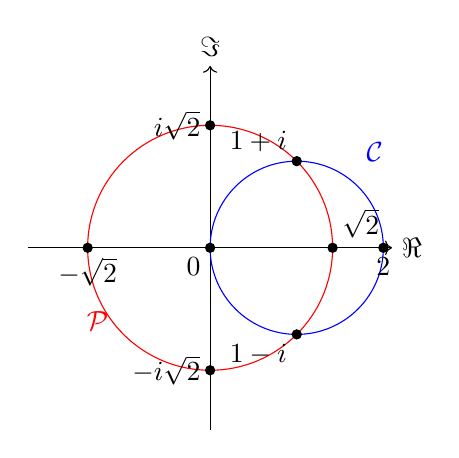
\begin{tikzpicture}[scale=1.1]
  \draw[->] (-2.1,0) -- (2.1,0) node[right] {$\Re$};
  \draw[->] (0,-2.1) -- (0,2.1) node[above] {$\Im$};
  \draw[blue] (1,0) circle (1);
  \draw[red] (0,0) circle (1.414);
  \filldraw (0,0) circle (1.5pt) node[below left] {$0$};
  \filldraw (2,0) circle (1.5pt) node[below] {$2$};
  \filldraw (1.414,0) circle (1.5pt) node[above right] {$\sqrt2$};
  \filldraw (-1.414,0) circle (1.5pt) node[below] {$-\sqrt2$};
  \filldraw (0,1.414) circle (1.5pt) node[left] {$i\sqrt2$};
  \filldraw (0,-1.414) circle (1.5pt) node[left] {$-i\sqrt2$};
  \filldraw (1,1) circle (1.5pt) node[above left] {$1+i$};
  \filldraw (1,-1) circle (1.5pt) node[below left] {$1-i$};
  \node[blue] at (1.9,1.1) {$\mathcal{C}$};
  \node[red] at (-1.3,-0.85) {$\mathcal{P}$};
\end{tikzpicture}
\caption{The two base-point circles (drawn for $p=2$): the critical
circle $\mathcal C=\{w:\|w-1\|=1\}$ (centre $1$, radius $1$, passing
through $0$ and $2$) and the prime circle
$\mathcal P=\{z:\|z\|^2=p\}$ (centre $0$, radius $\sqrt p$; where the
two-squares lattice points of the prime $p$ lie); the two circles meet at
$1\pm i$.}
\label{fig:circles}
\end{figure}

\section{Fold coordinates: four readings}
\label{sec:fold}

\paragraph{Phenomenon.} Rotating the axes of the standard complex plane
by $45^\circ$ gives two orthogonal coordinate axes $u$ and $v$ (constant
$\sqrt2/2=2^{-1/2}$). In these coordinates the imaginary axis
($\Re z=0$) presents itself as a $90^\circ$ fold: two straight arms run
out of $-1$ at $\pm45^\circ$, passing through $\pm i$ (drawn up to
$\pm i$); the fold (the union of the two rays) is homeomorphic to the
real axis. One and the same unit circle has one appearance per reading:
the standard complex plane, the $\pm45^\circ$ rotated frame, the
presentation reading in which each axis carries only the unit $1$, and
the fold reading (Figure~\ref{fig:four_views}).

\paragraph{Theorem/lemma.} Three verified results:
\begin{theorem}[Fold coordinates]
\label{thm:fold}
(i) Equivalence with the standard coordinates:
$\frac{u+v}{\sqrt2}=\Re z$, $\frac{u-v}{\sqrt2}=\Im z$
(\texttt{axis\_recovery\_re}, \texttt{axis\_recovery\_im}); the
coordinates determine the position uniquely (\texttt{axis\_unique});
modulus preservation $u^2+v^2=(\Re z)^2+(\Im z)^2$
(\texttt{axis\_norm\_sq\_preserving}); conversely every pair $(u,v)$
corresponds to some complex position (\texttt{axis\_exists}, simply
putting the standard coordinates back into the container).
(ii) The imaginary axis is the diagonal: $\Re z=0$ if and only if
$u+v=0$ (\texttt{fold\_imag\_axis\_diag}); the fold meets the imaginary
axis at $\pm i$ (\texttt{fold\_vertices\_are\_imag\_units}); the fold is
homeomorphic to the real axis (\texttt{foldArcHomeo}).
(iii) Triangle reading of the fold: the two legs each have length
$\sqrt2/2$; the hypotenuse corresponds to the length reading $|i|=1$ and
the value reading $[0,-1]$ (value $-1$); Pythagorean relation
$(\sqrt2/2)^2\cdot2=1^2$ (\texttt{fold\_tri\_pythagorean}); arm sum
$0.5i+0.5i=i$, value chain $i\cdot i=-1$
(\texttt{fold\_tri\_arms\_sum} etc.).
\end{theorem}

\paragraph{Hypotheses.} The fold is constructed only from standard facts
(Euler's identity $e^{i\pi}=-1$ gives the negative-side starting point,
rotation gives $\pm i$, direction $45^\circ$, length $\sqrt2$); it
contains no new mathematics; it is a restatement of the imaginary axis
(the fold meets the imaginary axis at $\pm i$,
\texttt{fold\_vertices\_are\_imag\_units}; the line generated by the two
intersection points is the imaginary axis,
\texttt{imag\_axis\_eq\_span\_fold\_vertices}). The fold and ``the native
straight axis in a raised dimension'' are two options at the presentation
layer: the straight axis raises the dimension by one more level and
produces no new machine-checkable content; the fold keeps the dimension
and makes explicit, and machine-checkable, the fact that in the standard
framework the two roots enter the plane differently ($\sqrt2$ stays on
the real axis, $\sqrt{-1}$ enters by raising the dimension). This paper
takes the fold; this is a choice at the presentation layer, stated openly
for the reader to judge. The fold reading comes from the author's
published representation framework \cite{zenodo, patbase}; only the
coordinate part of it is used here.

\paragraph{Lean formalization.} \texttt{EulerFoldImagAxis.lean}
(89 declarations) and \texttt{NativeAxisEquiv.lean} (11 declarations)
cover the items above; all 0 \texttt{sorry}, no axioms introduced.

\paragraph{Conclusion.} The complex plane acquires two mutually
convertible coordinate systems. Four correspondences follow (all
machine-checked): conjugation corresponds to swapping $u$ and $v$
(\texttt{fold\_conj\_swap}); the imaginary axis corresponds to the
diagonal $u+v=0$ (\texttt{fold\_imag\_axis\_diag}); the critical line
corresponds to the horizontal line $u+v=\sqrt2/2=2^{-1/2}$
(\texttt{fold\_critical\_line\_horiz}); real values correspond to the
fixed line of the swap (\texttt{fold\_real\_iff\_swap\_fixed}). The next
section takes the observation plane in these two coordinate systems
(\S\ref{sec:plane}).

\begin{figure}[ht]
\centering
% Four renderings of the same Euler-circle coordinate system, side by side.
% (a) the complex-plane view; (b) the same circle in the sin(±45°) u/v frame;
% (c) pat: u/v axes carry unit 1 only, values on the real axis (perpendicular);
% (d) the two pure axes twisted into three dimensions, orthogonality kept.
\begin{minipage}[t]{0.48\textwidth}\centering
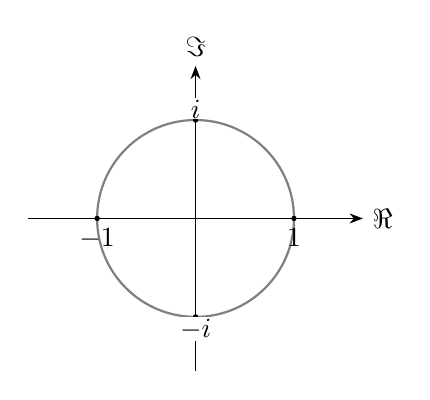
\begin{tikzpicture}[scale=1.25, >=Stealth]
  \draw[gray, thick] (0,0) circle (1);
  \draw[->] (-1.7,0) -- (1.7,0) node[right] {$\Re$};
  \draw[->] (0,-1.55) -- (0,1.55) node[above] {$\Im$};
  \filldraw (-1,0) circle (0.6pt) node[below] {$-1$};
  \filldraw (1,0) circle (0.6pt) node[below] {$1$};
  \filldraw (0,1) circle (0.6pt) node[above, fill=white, inner sep=0.5pt] {$i$};
  \filldraw (0,-1) circle (0.6pt) node[below, fill=white, inner sep=0.5pt] {$-i$};
\end{tikzpicture}
{\small (a) complex-plane view: standard $\Re$/$\Im$ axes, $\pm1$, $\pm i$, unit circle}
\end{minipage}\hfill
\begin{minipage}[t]{0.48\textwidth}\centering
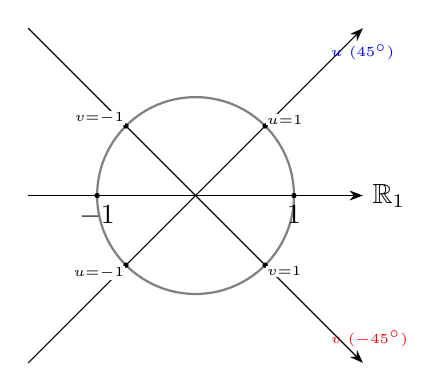
\begin{tikzpicture}[scale=1.25, >=Stealth]
  \draw[gray, thick] (0,0) circle (1);
  \draw[->] (-1.7,0) -- (1.7,0) node[right] {$\R_1$};
  \draw[->] (-1.7,-1.7) -- (1.7,1.7) node[very near end, above right, font=\tiny, blue] {$u$ ($45^\circ$)};
  \draw[->] (-1.7,1.7) -- (1.7,-1.7) node[very near end, below right, font=\tiny, red] {$v$ ($-45^\circ$)};
  \filldraw (-1,0) circle (0.6pt) node[below] {$-1$};
  \filldraw (1,0) circle (0.6pt) node[below] {$1$};
  \filldraw (0.707,0.707) circle (0.6pt) node[above right, font=\tiny, fill=white, inner sep=0.5pt] {$u{=}1$};
  \filldraw (-0.707,-0.707) circle (0.6pt) node[below left, font=\tiny, fill=white, inner sep=0.5pt] {$u{=}{-}1$};
  \filldraw (0.707,-0.707) circle (0.6pt) node[below right, font=\tiny, fill=white, inner sep=0.5pt] {$v{=}1$};
  \filldraw (-0.707,0.707) circle (0.6pt) node[above left, font=\tiny, fill=white, inner sep=0.5pt] {$v{=}{-}1$};
\end{tikzpicture}
{\small (b) the same circle in the $\pm45^\circ$ rotated frame: the $u$/$v$ axes and their unit points $u{=}\pm1$, $v{=}\pm1$}
\end{minipage}\par\vspace{8pt}
\begin{minipage}[t]{0.48\textwidth}\centering
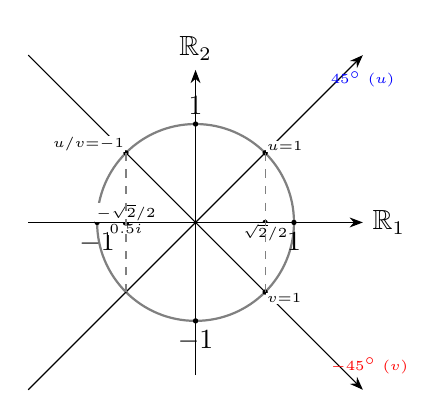
\begin{tikzpicture}[scale=1.25, >=Stealth]
  \draw[gray, thick] (0,0) circle (1);
  \draw[->] (-1.7,0) -- (1.7,0) node[right] {$\R_1$};
  \draw[->] (0,-1.55) -- (0,1.55) node[above] {$\R_2$};
  \filldraw (-1,0) circle (0.6pt) node[below] {$-1$};
  \filldraw (1,0) circle (0.6pt) node[below] {$1$};
  \filldraw (0,1) circle (0.6pt) node[above] {$1$};
  \filldraw (0,-1) circle (0.6pt) node[below] {$-1$};
  \draw[->] (-1.7,-1.7) -- (1.7,1.7) node[very near end, above right, font=\tiny, blue] {$45^\circ\ (u)$};
  \draw[->] (-1.7,1.7) -- (1.7,-1.7) node[very near end, below right, font=\tiny, red] {$-45^\circ\ (v)$};
  % no numeric scales on the axes: each axis carries only the unit point 1 (pat: all axes are 1)
  \filldraw (-0.707,0) circle (0.8pt) node[below, font=\tiny, fill=white, inner sep=0.5pt] {$0.5i$};
  \filldraw (-0.707,0) circle (0.8pt) node[above, font=\tiny, fill=white, inner sep=0.5pt] {$-\sqrt2/2$};
  \filldraw (0.707,0) circle (0.6pt) node[below, font=\tiny, fill=white, inner sep=0.5pt] {$\sqrt2/2$};
  \filldraw (0.707,0.707) circle (0.6pt) node[above right, font=\tiny, fill=white, inner sep=0.5pt] {$u{=}1$};
  \filldraw (0.707,-0.707) circle (0.6pt) node[below right, font=\tiny, fill=white, inner sep=0.5pt] {$v{=}1$};
  \filldraw (-0.707,0.707) circle (0.6pt) node[above left, font=\tiny, fill=white, inner sep=0.5pt] {$u/v{=}{-}1$};
  \draw[dashed, gray] (0.707,0.707) -- (0.707,0);
  \draw[dashed, gray] (0.707,-0.707) -- (0.707,0);
  \draw[dashed, gray] (-0.707,0.707) -- (-0.707,0);
  \draw[dashed, gray] (-0.707,-0.707) -- (-0.707,0);
\end{tikzpicture}
{\small (c) presentation reading: the $u$/$v$ axes (unit $1$, no numbers on the axes); the readings on the real axis $\sqrt2/2$ (the $+1$ reading) and $0.5i$ (the $-1$ reading, the vertical component of the arm), with feet at $\pm\sqrt2/2$}
\end{minipage}\hfill
\begin{minipage}[t]{0.48\textwidth}\centering
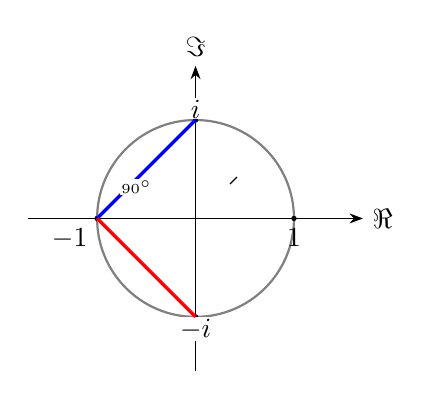
\begin{tikzpicture}[scale=1.25, >=Stealth]
  \draw[gray, thick] (0,0) circle (1);
  \draw[->] (-1.7,0) -- (1.7,0) node[right] {$\Re$};
  \draw[->] (0,-1.55) -- (0,1.55) node[above] {$\Im$};
  \filldraw (-1,0) circle (0.6pt) node[below left] {$-1$};
  \filldraw (1,0) circle (0.6pt) node[below] {$1$};
  \filldraw (0,1) circle (0.6pt) node[above, fill=white, inner sep=0.5pt] {$i$};
  \filldraw (0,-1) circle (0.6pt) node[below, fill=white, inner sep=0.5pt] {$-i$};
  \draw[very thick, blue] (-1,0) -- (0,1);
  \draw[very thick, red] (-1,0) -- (0,-1);
  \draw (0.35,0.35) -- (0.42,0.42);
  \node[font=\tiny, fill=white, inner sep=0.5pt] at (-0.6,0.32) {$90^\circ$};
\end{tikzpicture}
{\small (d) the $90^\circ$ fold starting at $-1$: two straight arms through $\pm i$ (drawn up to $\pm i$)}
\end{minipage}
\caption{One unit circle under four readings: (a) complex-plane view
(standard $\Re$/$\Im$ axes, $\pm1$, $\pm i$); (b) the same circle in the
$\pm45^\circ$ rotated frame --- the $u$/$v$ axes and their unit points
$u{=}\pm1$, $v{=}\pm1$; (c) presentation reading: the $u$/$v$ axes carry
only the unit $1$, while every value appears on the real axis through
perpendicular projection --- the readings are $\sqrt2/2$ (the $+1$
reading) and $0.5i$ (the $-1$ reading, the vertical component of the
arm), with feet at $\pm\sqrt2/2$; (d) the $90^\circ$ fold starting at
$-1$: two straight arms through $\pm i$ (drawn up to $\pm i$). All radii
are $1$; schematic.}
\label{fig:four_views}
\end{figure}

\section{The observation plane: three coordinate properties}
\label{sec:plane}

\paragraph{Phenomenon.} For a single point, ``is it on the critical
line'' is answered by one number: the distance to the critical line
$\Re s-1/2$. The position along the line $\Im s$ takes no part in this
judgement. The observation plane takes two axes: axis~1 along the
critical line, reading $\sqrt2\,\Im s$; axis~2 perpendicular to the
critical line, reading $\sqrt2(\Re s-\frac12)$, whose origin is placed on
the critical line. The projection is the reading of axis~2, written
\[
  d(s)=\texttt{foldObsProj}(s)=u(s)+v(s)-\frac{\sqrt2}{2}
      =\sqrt2\Big(\Re s-\frac12\Big).
\]

\paragraph{Theorem/lemma.} Three coordinate properties are verified:
\begin{theorem}[Projection]
\label{thm:plane}
(1) The projection collapses to a point: if $\Re s=1/2$ then $d(s)=0$,
i.e.\ the whole critical line is mapped to a single point on axis~2
(\texttt{critical\_projects\_to\_axis2\_point}; fold-coordinate version
\texttt{fold\_critical\_projects\_point}).
(2) Faithfulness: conversely, $d(s)=0$ if and only if $\Re s=1/2$, for
all $s\in\C$, not only in the strip
(\texttt{only\_critical\_projects\_to\_point};
\texttt{fold\_projection\_point\_iff\_critical}).
(3) No self-reference: the definition of $d$ uses only the fold
coordinates, not $\zt$
(\texttt{foldObsProj\_independent\_of\_zeta}; standard version
\texttt{obsProj\_independent\_of\_zeta}).
\end{theorem}

\paragraph{Hypotheses.} Properties (1)--(3) hold for every point, zero
or not. They are coordinate facts and carry no information about zeros;
the strip condition $0<\Re s<1$ is used only in \S\ref{sec:complete},
when zeros are judged.

\paragraph{Lean formalization.} \texttt{AxisExactObservation.lean}
(18 declarations) and \texttt{FoldObservation.lean} contain the items
above; 0 \texttt{sorry}.

\paragraph{Conclusion.} The projection is a qualified decision tool: the
reading needed for the judgement exists, and its definition is
independent of $\zt$. The judgement also needs a reading on the side of
zero-ness, given in the next section (\S\ref{sec:anchors}).

\section{The projection characterization of zero-ness: two value-range
anchors}
\label{sec:anchors}

\paragraph{Phenomenon.} The judgement needs to answer another question:
given a point $s$, how do we know that it is a zero of $\zt$. Applying
the fold formula to the value $\zt(s)$ produces two real components
\[
  U(s)=\frac{\sqrt2}{2}\big(\Re\zt(s)+\Im\zt(s)\big),
  \qquad
  V(s)=\frac{\sqrt2}{2}\big(\Re\zt(s)-\Im\zt(s)\big).
\]
At a zero both components vanish simultaneously.

\paragraph{Theorem/lemma.} Three verified results:
\begin{theorem}[Value-range anchors]
\label{thm:anchors}
(1) Value anchors: $U+V=\sqrt2\,\Re\zt(s)$,
$U-V=\sqrt2\,\Im\zt(s)$ (\texttt{zeta\_fold\_sum\_re},
\texttt{zeta\_fold\_diff\_im}).
(2) The components are invertible: $(U,V)$ recovers $\zt(s)$
(\texttt{zeta\_fold\_invertible}), and $\zt(s)=0$ if and only if
$U(s)=V(s)=0$ (\texttt{zeta\_fold\_zero\_iff}).
(3) A zero forces both anchors to vanish: if $\zt(\rho)=0$ then
$U(\rho)+V(\rho)=0$ and $U(\rho)-V(\rho)=0$
(\texttt{zeta\_fold\_dual\_proj\_zero\_of\_zero}).
\end{theorem}

\paragraph{Hypotheses.} These are pointwise identities; no extra
hypotheses are needed; $\zt(\rho)=0$ is the premise when zero-ness is
discussed.

\paragraph{Lean formalization.} \texttt{FoldObservation.lean}:
\texttt{zetaFoldU}, \texttt{zetaFoldV},
\texttt{zeta\_fold\_invertible}, \texttt{zeta\_fold\_zero\_iff},
\texttt{zeta\_fold\_sum\_re}, \texttt{zeta\_fold\_diff\_im},
\texttt{zeta\_fold\_dual\_proj\_zero\_of\_zero}; 0 \texttt{sorry}.

\paragraph{Conclusion.} Zero-ness is fully characterized by the two
projection components of the value; combined with the coordinate reading
of \S\ref{sec:plane}, this yields the judgement completeness of the next
section (\S\ref{sec:complete}).

\section{Judgement completeness: the weak assertion}
\label{sec:complete}

\paragraph{Phenomenon.} Now combine the two sides: zero-ness lives in
the value components $(U,V)$, being on the critical line lives in the
axis-2 reading $d$, and the position along the line never appears. One
may say: the information that remains after the projection drops axis~1
is enough to decide whether a zero lies on the critical line.

\paragraph{Theorem/lemma.}
\begin{theorem}[Judgement completeness; verified]
\label{thm:weak}
For a zero $\rho$ in the strip ($\zt(\rho)=0$, $0<\Re\rho<1$):
\[
  \Re\rho=\tfrac12
    \iff d(\rho)=0
    \iff \big(U(\rho)=0 \wedge V(\rho)=0 \wedge d(\rho)=0\big).
\]
(\texttt{projection\_zero\_line\_complete}, FoldObservation.lean; the
strip factor $2^{-\rho}\ne1$ is verified separately; supporting item
\texttt{fold\_zero\_judgement\_preserved}.)
\end{theorem}

\paragraph{Hypotheses.} The result of this section is usually called the
weak assertion: it states the completeness of the judgement, not that the
conclusion holds. ``Complete'' means that the judgement sentence and the
projection form are true together and false together, derivable in both
directions; it does not mean that ``the reading equals zero'' holds.
Table~\ref{tab:status} below separates the three kinds of statements:
the first two rows are verified equivalences, the third row is the
statement to be proved. The coordinate properties hold for every point,
independent of zeros; judgement completeness holds for zeros, with
$\zt(\rho)=0$ as the premise. Neither of them gives us the conclusion
``all readings vanish'': that requires the universal quantifier over all
zeros (\S\ref{sec:equivalence}).

\begin{table}[h]
\centering
\begin{tabular}{@{}>{\raggedright\arraybackslash}p{0.20\textwidth}@{\quad}>{\raggedright\arraybackslash}p{0.53\textwidth}@{\quad}>{\raggedright\arraybackslash}p{0.19\textwidth}@{}}
\hline
Statement & Content & Status \\
\hline
Coordinate properties & the critical line maps to a point; no other point maps there; definition free of $\zt$ & verified (\S\ref{sec:plane}) \\
Judgement completeness & zeros in the strip: on the line iff $d=0$; zero-ness characterized by the two value anchors & verified (\S\ref{sec:complete}) \\
Universal reading & every zero in the strip satisfies $d=0$ & open; equivalent to the Riemann hypothesis (\S\ref{sec:equivalence}) \\
\hline
\end{tabular}
\caption{The three kinds of statements and their verification status.}
\label{tab:status}
\end{table}

\paragraph{Lean formalization.} \texttt{FoldObservation.lean}:
\texttt{projection\_zero\_line\_complete} etc.; 0 \texttt{sorry}.

\paragraph{Conclusion.} The work at the judgement layer is complete here:
the criterion is lossless. What judgement each individual zero yields is
the universal statement of the next section.

\section{Equivalent restatements: the Riemann hypothesis as a reading
constraint}
\label{sec:equivalence}

\paragraph{Phenomenon.} Substituting a zero into the judgement of
\S\ref{sec:complete} yields a universal statement: the projection reading
of every zero in the strip is zero. This statement is true exactly when
the Riemann hypothesis is.

\paragraph{Theorem/lemma.}
\begin{theorem}[Reading form; verified]
\label{thm:equiv}
The Riemann hypothesis (\texttt{rh\_classical}) is equivalent to
\[
  \forall s:\ 0<\Re s<1 \ \wedge\ \Im s\ne0\ \wedge\ \zt(s)=0
  \ \Longrightarrow\ \texttt{foldObsProj}(s)=0 .
\]
(\texttt{fold\_rh\_iff\_axis\_form}, FoldObservation.lean;
standard-coordinate version \texttt{rh\_iff\_axis\_form},
AxisExactObservation.lean.)
\end{theorem}
Moreover several further equivalent formulations (equivalent
restatements of the Riemann hypothesis have many precedents in the
literature, e.g.\ \cite{lagarias2002}) are verified:
\begin{itemize}
\item Counting form: the Riemann hypothesis holds if and only if the
number of zeros on the line equals the number of zeros in the strip
(\texttt{rh\_iff\_N0\_eq\_N}; the version for each height $T$ is
\texttt{count\_eq\_iff\_all\_on\_line}, ValueBridge.lean), whose
geometric background is the argument-principle rectangle
(Figure~\ref{fig:rect});
\item Common-vertical-line form: the Riemann hypothesis holds if and
only if all zeros in the strip lie on one single vertical line
(\texttt{common\_line\_iff\_RH}, probe CommonLineCheck.lean); here the
``line'' can only be $\Re=1/2$, forced by the reflection pairing;
\item Contrapositive form: the hypothesis fails if and only if an
off-line zero in the strip exists
(\texttt{rh\_failure\_iff\_offline\_common\_zero}).
\end{itemize}

As a positioning, Table~\ref{tab:neighbors} places the nearest-neighbour
forms side by side with the difference from this draft (the increment of
this draft is in the two layers of machine verification and calibration).

\begin{center}
\begin{tabular}{@{}>{\raggedright\arraybackslash}p{0.23\textwidth}@{\quad}>{\raggedright\arraybackslash}p{0.28\textwidth}>{\raggedright\arraybackslash}p{0.40\textwidth}@{}}
\hline
Relation form & Source & Difference from this draft \\
\hline
Counting form: number of zeros on the line equals number of zeros in the strip & classical corollary of the argument principle (textbook \cite{titchmarsh}) & this draft lists it alongside the reading form, and machine-verifies that the two are true together \\
Horizontal monotonicity $\Leftrightarrow$ Riemann hypothesis & Sondow--Dumitrescu \cite{sondow2010}; Matiyasevich--Saidak--Zvengrowski \cite{msz2014} & the form is a monotonicity of moduli; the form in this draft is the coordinate reading $d$ \\
Elementary criterion (divisor function) & Lagarias \cite{lagarias2002} & the object is the divisor function, a different class from coordinate readings \\
Equivalence involving $\zt'$ & Speiser \cite{speiser} & the object is the derivative \\
Proportion of zeros on the line ($1/3$, $2/5$) & Levinson \cite{levinson1974}; Conrey \cite{conrey1989} & partial results, not equivalences \\
\hline
\end{tabular}
\end{center}
\captionof{table}{Positioning relative to the nearest neighbours (all
known results).}\label{tab:neighbors}
\vspace{6pt}

\paragraph{Hypotheses.} These equivalences are standard pointwise
translations; no hypotheses are added. Watch the quantifier: the version
truncated at height $|\Im|\le T$ (saying ``the zeros in the strip with
height at most $T$ are collinear'') is a finite statement and does not
imply the Riemann hypothesis; only the universal version is equivalent
to it.

\paragraph{Lean formalization.} \texttt{AxisExactObservation.lean},
\texttt{FoldObservation.lean}, \texttt{CommonLineCheck.lean} and
\texttt{ValueBridge.lean} cover the items above; 0 \texttt{sorry}.

\paragraph{Conclusion.} The Riemann hypothesis can be restated as one
sentence about readings: the projection reading of every zero in the
strip is zero. The restatement is verified; the sentence itself remains
open; the structural diagnosis of the gap is in the next section
(\S\ref{sec:diag}).

\begin{remark}[Two-level calibration of judgement]
\label{rem:levels}
Reading the verified results side by side gives the following facts.
(i) Individual level: for each zero in the strip, ``on the critical
line'' and ``reading $d=0$'' are true together and false together, and
the judgement does not refer to $\zt$ (\S\ref{sec:complete}).
(ii) Universal level: ``all readings of zeros in the strip are zero'' is
true together with the Riemann hypothesis (\S\ref{sec:equivalence}).
(iii) Intermediate: the common intermediate candidate ``flip count
equals winding count'' ($K_{\mathrm{flip}}=K_{\mathrm{wind}}$) does not
constitute an independent level --- it is true together with the
universal statement of (ii) (counting equivalence; its sufficient
direction is verified by the conditional assembly, \S\ref{sec:diag}).
Hence judgement in this framework has only two levels: the individual
judgement is complete, the universal judgement is open, and there is no
independent intermediate level. Also (standard observation, KNOWN, not
relied upon in this paper): the negative direction of the universal
statement has a finite certificate --- a single off-line zero can be
exhibited by an isolation region and a zero count (zero counting rests
on the argument principle \cite{titchmarsh}); the positive direction has
no purely instance-by-instance finite verification path, and must give
an argument covering all cases.
\end{remark}

\begin{figure}[h]
\centering
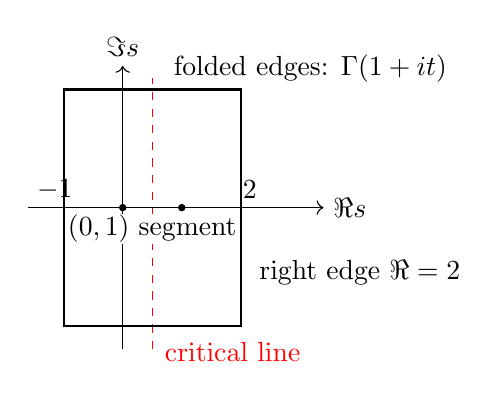
\begin{tikzpicture}[scale=0.75]
  \draw[->] (-1.6,0) -- (3.4,0) node[right] {$\Re s$};
  \draw[->] (0,-2.4) -- (0,2.4) node[above] {$\Im s$};
  \draw[dashed,red] (0.5,-2.4) -- (0.5,2.2);
  \node[red, anchor=west] at (0.55,-2.45) {critical line};
  \draw[thick] (-1,2) -- (2,2) -- (2,-2) -- (-1,-2) -- cycle;
  \node at (2.15,0.3) {$2$};
  \node at (-1.15,0.3) {$-1$};
  \filldraw (0,0) circle (1.5pt);
  \filldraw (1,0) circle (1.5pt);
  \node[below=2pt, fill=white, inner sep=0.5pt] at (0.5,0) {$(0,1)$ segment};
  \node[anchor=west] at (2.15,-1.1) {right edge $\Re=2$};
  \node[anchor=west] at (0.7,2.35) {folded edges: $\GG(1+it)$};
\end{tikzpicture}
\caption{The argument-principle rectangle, with vertices $-1\pm iT$,
$2\pm iT$ (drawn here for $T=2$): the bottom edge $[-1,2]$ (false-real-axis
assembly: the negative half-plane is folded, via the functional equation,
into the positive series region $\Re s>1$), the right edge $\Re s=2$
(bounded by $\sum n^{-2}$), and the top and left edges folded by the
functional equation. The geometric background of the counting
equivalence.}
\label{fig:rect}
\end{figure}

\section{Structural diagnosis of the remaining step, and its boundary}
\label{sec:diag}

\paragraph{Phenomenon.} ``No off-line zeros'' cannot so far be derived
from the existing structures; splitting the route ``an off-line zero
yields a contradiction'' gives three verified structural diagnoses.
(1) The bridge family fails on the off-line orbit: if $\rho$ is an
off-line zero in the strip, then $\rho$, $\bar\rho$, $1-\rho$,
$1-\bar\rho$ are all zeros (reflection pairing,
\texttt{zeta\_zero\_offline\_pair}, proof.lean); bridges whose input
condition is $\zt\ne0$ (Euler product, ratio, phase) are unusable
anywhere on this orbit. At a zero the odd and even parts vanish
simultaneously, and the single-lift ratio is $0/0$
(\texttt{self\_reference\_resolved}); the difference structure, which is
the phase ratio, is well-defined but carries no information about $\zt$
(\texttt{phase\_ratio\_unit}).
(2) Linear observations cannot distinguish: the existing observables are
linear or algebraic reorganizations of coordinates and preserve the zero
set; under the assumption ``an off-line zero exists'', the eight-point
signature (\texttt{eight\_point\_observation}) and the first-order
skeleton (\texttt{offline\_T\_coord\_skeleton}, TCoordOffline.lean) are
all consistent with it and produce no contradiction.
(3) The counting form is circular: writing the contradiction as a count,
the only hypothesis left is ``flip count equals winding count''
($K_{\mathrm{flip}}=K_{\mathrm{wind}}$), which is precisely the counting
form of the Riemann hypothesis.

\paragraph{Theorem/lemma.}
\begin{theorem}[Conditional assembly; verified]
\label{thm:assembly}
Given the bridges on both sides of the count and the hypothesis
$K_{\mathrm{flip}}=K_{\mathrm{wind}}$ (in Lean: the hypothesis
\texttt{hflip\_eq} of \texttt{value\_bridge\_assembly}), there are no
off-line zeros (\texttt{value\_bridge\_assembly}, ValueBridge.lean; the
contradiction is closed by \texttt{value\_bridge\_contradiction}). That
is, the missing step of the chain is written as one counting identity;
this identity is open, and it is equivalent to the Riemann hypothesis
(the boundary of the reduction chain; see \S\ref{sec:equivalence}).
\end{theorem}

\paragraph{Hypotheses.} The input of the contradiction argument is
``an off-line zero in the strip exists''. Further, classical results for
contrast (KNOWN): the zero-free region (de la Vall\'ee Poussin) excludes
zeros on the $\sigma\to1$ side, but only up to a logarithmic distance
\cite{hadamard1896, delavallee1899}; Hardy proved that there are
infinitely many zeros on the critical line \cite{hardy1914}; Levinson
and Conrey give positive proportions on the line
\cite{levinson1974, conrey1989}; Speiser gives an equivalent form
involving $\zt'$ \cite{speiser}; and Davenport--Heilbronn show that the
functional equation and an Euler-product-type structure alone do not
suffice to force zeros onto the line: Dirichlet series of the same type
can have off-line zeros \cite{davenport}.

\paragraph{Lean formalization.} The items above are covered by the files
\texttt{ValueBridge.lean}, \texttt{TCoordOffline.lean},
\texttt{FoldObservation.lean} and \texttt{proof.lean}; each file is at 0
\texttt{sorry}.

\paragraph{Conclusion.} The remaining step is not the gap of a single
lemma but a universal constraint equivalent to the Riemann hypothesis;
the rigid projection that links an off-line zero to a contradiction is
called a generator in this paper. This paper does not make the
construction of the generator a project; it only records the existing
structural facts and the boundary clearly.

\section{Verification record and reproduction}
\label{sec:verify}

\paragraph{Phenomenon.} Every declaration cited in this paper compiles
under one tool chain, and can be checked independently.

\paragraph{Record.} Environment: Lean~4.32.2 and mathlib (revision
905b95818e) \cite{mathlib, lean}. All 0 error, 0 \texttt{sorry}; no
axioms beyond those of mathlib are introduced; the files cited here do
not depend on the only explicit axiom of the companion work (the Pat0
absorbing rule, located in the phase-locking chain). The declaration
count counts theorems $+$ lemmas $+$ defs, not instances:

\begin{center}
\begin{tabular}{lr}
\hline
File & Declarations \\
\hline
\texttt{AxisExactObservation.lean} & 18 \\
\texttt{FoldObservation.lean} & 90 \\
\texttt{NativeAxisEquiv.lean} & 11 \\
\texttt{EulerFoldImagAxis.lean} & 89 \\
\texttt{ValueBridge.lean} & 25 \\
\texttt{PreciseMigration.lean} & 20 \\
\texttt{CommonLineCheck.lean} (probe) & 2 \\
\hline
\end{tabular}
\end{center}
\captionof{table}{Files and declaration counts.}\label{tab:files}
\vspace{6pt}

The count of the assembly chain in the companion tree: fourteen layers,
284 declarations in total (with cross-layer repeats; the main proof file
\texttt{proof.lean} holds 231 under the same convention), 0
\texttt{sorry} (Figure~\ref{fig:map}). The last row of
Table~\ref{tab:files} is taken from the probe directory (an independently
placed check item); the other files belong to the paper's companion
tree. Reproduction: inside that tree run
\texttt{lake env lean ../../探针\_20261010/CommonLineCheck.lean}
(expected exit 0); library-level checks use \texttt{build.sh} and
\texttt{check\_sorry.py}.

\paragraph{Hypotheses.} Version and caches are fixed as recorded; the
numbers in Table~\ref{tab:files} agree with the declaration counts of the
files (convention as above).

\paragraph{Lean formalization.} See Table~\ref{tab:files}; all 0
\texttt{sorry}.

\paragraph{Conclusion.} The chain of evidence can be checked
independently.

\begin{figure}[h]
\centering
\begin{minipage}{\textwidth}\centering
\resizebox{\textwidth}{!}{%
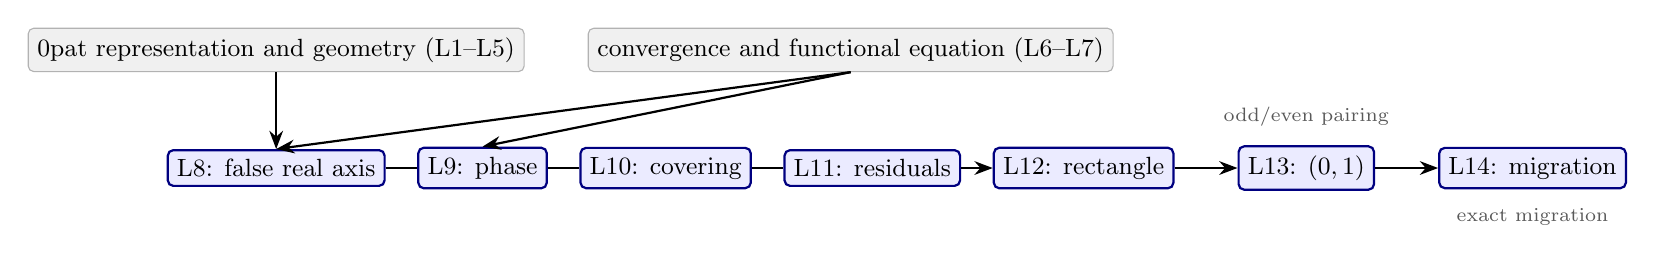
\begin{tikzpicture}[
  bg/.style={fill=gray!12, draw=gray!60, rounded corners=2pt},
  core/.style={fill=blue!8, draw=blue!50!black, rounded corners=2pt, thick},
  edge/.style={-{Stealth}, thick},
  lab/.style={font=\scriptsize, text=gray!70!black}]
  % background presentation layers
  \node[bg] (bg) at (0,0) {\small 0pat representation and geometry (L1--L5)};
  \node[bg, right=8mm of bg] (fe) {\small convergence and functional equation (L6--L7)};
  % analytic core chain
  \node[core] (L8) at (0,-1.5) {\small L8: false real axis};
  \node[core, right=4mm of L8] (L9) {\small L9: phase};
  \node[core, right=4mm of L9] (L10) {\small L10: covering};
  \node[core, right=4mm of L10] (L11) {\small L11: residuals};
  \node[core, right=4mm of L11] (L12) {\small L12: rectangle};
  \node[core, right=8mm of L12] (L13) {\small L13: $(0,1)$};
  \node[core, right=8mm of L13] (L14) {\small L14: migration};
  % arrows
  \draw[edge] (bg.south) -- (L8.north);
  \draw[edge] (fe.south) -- (L8.north);
  \draw[edge] (fe.south) -- (L9.north);
  \draw[edge] (L8) -- (L9) -- (L10) -- (L11) -- (L12);
  % annotations
  \node[lab, above=1.2mm of L13] {odd/even pairing};
  \draw[edge] (L12.east) -- (L13.west);
  \draw[edge] (L13) -- (L14);
  \node[lab, below=1.2mm of L14] {exact migration};
\end{tikzpicture}}
\end{minipage}
\caption{The fourteen layers of the assembly chain and the dependency
flow (overview of the assembly chain in the companion tree); the
declarations cited in this paper about the observation plane lie in L8
(false real axis) and in the migration layer L14.}
\label{fig:map}
\end{figure}

\section{Conclusion}
\label{sec:conclusion}

\paragraph{Phenomenon.} The paper has two parts. One part consists of
verified equivalences and structures: the three coordinate properties of
the observation plane, judgement completeness, and the reading form of
the Riemann hypothesis. The other part is a universal constraint that
remains open: the projection reading of every zero in the strip is zero.

\paragraph{Theorem (summary).} The Riemann hypothesis is equivalent to
``the projection reading of every zero in the strip is zero''
(\texttt{fold\_rh\_iff\_axis\_form}); judgement completeness is
\texttt{projection\_zero\_line\_complete}; the reduction boundary writes
``no off-line zeros'', ``all readings vanish'' and ``counting agrees''
as one and the same thing.

\paragraph{Hypotheses (boundary).} This paper does not claim to prove or
disprove the Riemann hypothesis, nor does it make metamathematical
assertions about provability; classical results that are not
machine-verified are marked KNOWN; the coordinate properties and
judgement completeness (\S\ref{sec:plane} to \S\ref{sec:complete}) apply
to all points or to individual zeros, and are statements of a different
strength from the universal constraint (\S\ref{sec:equivalence}); they
must not be conflated.

\paragraph{Lean formalization.} All 0 error, 0 \texttt{sorry}; files and
counts in \S\ref{sec:verify}.

\paragraph{Conclusion.} The Riemann hypothesis can be placed precisely
on a machine-verified observation plane: it is equivalent to ``all
readings of zeros are zero''. The judgement layer is complete; the
statement itself remains open. Further progress requires constructing a
generator on the plane (see \S\ref{sec:diag}); everything before this
step has been organized in this paper.

\begin{thebibliography}{99}
\bibitem{riemann1859}
B.~Riemann, Ueber die Anzahl der Primzahlen unter einer gegebenen
Gr\"osse, \emph{Monatsberichte der K\"oniglich Preussischen Akademie
der Wissenschaften zu Berlin} (1859), 671--680.
\bibitem{hadamard1896}
J.~Hadamard, Sur la distribution des z\'eros de la fonction
$\zeta(s)$ et ses cons\'equences arithm\'etiques, \emph{Bull.\ Soc.\
Math.\ France} \textbf{24} (1896), 199--220.
\bibitem{delavallee1899}
C.-J. de la Vall\'ee Poussin, Recherches analytiques sur la th\'eorie
des nombres premiers, \emph{Ann.\ Soc.\ Sci.\ Bruxelles} \textbf{21}
(1897), 183--256 and 281--397.
\bibitem{hardy1914}
G.~H. Hardy, Sur les z\'eros de la fonction $\zeta(s)$ de Riemann,
\emph{C.\ R.\ Acad.\ Sci.\ Paris} \textbf{158} (1914), 1012--1014.
\bibitem{speiser}
A.~Speiser, Geometrisches zur Riemannschen Zetafunktion,
\emph{Math.\ Ann.} \textbf{110} (1934), 514--521.
\bibitem{levinson1974}
N.~Levinson, More than one third of the zeros of Riemann's
zeta-function are on $\sigma=1/2$, \emph{Advances in Math.}
\textbf{13} (1974), 383--436.
\bibitem{conrey1989}
J.~B. Conrey, More than two fifths of the zeros of the Riemann zeta
function are on the critical line, \emph{J.\ Reine Angew.\ Math.}
\textbf{399} (1989), 1--26.
\bibitem{davenport}
H.~Davenport and H.~Heilbronn, On the zeros of certain Dirichlet
series, \emph{J.\ London Math.\ Soc.} \textbf{11} (1936), 181--185
and 307--312.
\bibitem{titchmarsh}
E.~C. Titchmarsh, \emph{The Theory of the Riemann Zeta-Function},
2nd ed., Oxford University Press, 1986.
\bibitem{edwards1974}
H.~M. Edwards, \emph{Riemann's Zeta Function}, Academic Press, 1974
(reprinted Dover, 2001).
\bibitem{ivic1985}
A.~Ivi\'c, \emph{The Riemann Zeta-Function: Theory and Applications},
Wiley, 1985.
\bibitem{lagarias2002}
J.~C. Lagarias, An elementary problem equivalent to the Riemann
hypothesis, \emph{Amer.\ Math.\ Monthly} \textbf{109} (2002), 534--543.
\bibitem{mathlib}
The mathlib community, \emph{mathlib4}, Lean repository,
revision 905b95818e, \url{https://github.com/leanprover-community/mathlib4}.
\bibitem{lean}
L.~de Moura, S.~Kong, J.~Avigad, F.~van Doorn, and J.~von Raumer,
The Lean theorem prover (system description), in \emph{CADE-25},
LNCS \textbf{9195}, Springer, 2015, pp.~378--388.
\bibitem{patbase}
Y.~Wang, \emph{Empirical Foundations of Pat: Transformer OOD Observations,
Structural Laws, and Machine-Checked Continuum Theorems}, 2026, submitted
for publication; framework basepaper of the 0pat release, containing the
machine-verified continuum closure theorems R150--R151 (the continuum
$[0,2\pi]$ is the closure of the countable pat grid). Framework release
v1: DOI
\href{https://doi.org/10.5281/zenodo.22038154}{10.5281/zenodo.22038154}.
\bibitem{zenodo}
Y.~Wang, \emph{Formalizing the Riemann Direction Unified Observation
under Logical Completeness Theory --- basepoint-relative 0pat
representation}, 2026. DOI:
\href{https://doi.org/10.5281/zenodo.22038154}{10.5281/zenodo.22038154}
(the framework release); the 0pat Exercise XXXVII revision packages are
recorded at \href{https://doi.org/10.5281/zenodo.22039506}{10.5281/zenodo.22039506},
\href{https://doi.org/10.5281/zenodo.22044557}{10.5281/zenodo.22044557}, and
\href{https://doi.org/10.5281/zenodo.22044634}{10.5281/zenodo.22044634}.
\bibitem{sondow2010}
J.~Sondow and C.~Dumitrescu, A monotonicity property of Riemann's xi
function and a reformulation of the Riemann hypothesis, \emph{Period.\
Math.\ Hungar.} \textbf{60} (2010), 37--40.
\bibitem{msz2014}
Yu.~Matiyasevich, F.~Saidak, and P.~Zvengrowski, Horizontal monotonicity
of the modulus of the zeta function, $L$-functions, and related
functions, \emph{Acta Arith.} \textbf{166} (2014), 189--200.
\end{thebibliography}

\end{document}
